\documentclass{aa}

\usepackage{graphicx}
\usepackage{float}
\usepackage[varg]{txfonts}
\usepackage[breaklinks=true]{hyperref}
\usepackage{booktabs}
\usepackage{amsmath}
\usepackage[utf8]{inputenc}
\usepackage{url}

\hypersetup{
  colorlinks=true,
  linkcolor=blue,
  urlcolor=cyan,
  pdftitle={Are galaxies in compact groups special? Online supplementary material}
}

\newcommand{\CB}{Control\textsubscript{4B}}
\newcommand{\CC}{Control\textsubscript{4C}}
\newcommand{\CG}{CG\textsubscript{4}}
\newcommand{\RG}{RG\textsubscript{4}}
\graphicspath{{figures/}}

\renewcommand{\thefigure}{S.\arabic{figure}}

\begin{document}
















\title{Are galaxies in compact groups special?\\Online supplementary material}
\author{Matthieu Tricottet \and Gary A. Mamon \and Eugenia D\'iaz-Gim\'enez}
\date{}
\maketitle

This supplement contains the distributional and pooled-model diagnostics moved out of the article for editorial economy. It uses the same samples, definitions, and fitted quantities as the article; no additional scientific claims are introduced here.

\section{Star-forming and quenched sequence residuals}

Star-forming \CG{} galaxies do not sit off the star-forming main sequence (SFMS). Relative to an order-2 polynomial SFMS fitted to the star-forming galaxies of the SDSS reference sample, the median residual of \CG{} star-forming galaxies exceeds that of the controls by \(0.056\), \(0.058\), and \(0.046\) dex for \CB{}, \CC{}, and \RG{} (68\% group-bootstrap intervals \([0.03, 0.10]\), \([0.04, 0.10]\), and \([-0.04, 0.10]\); sign-crossing \(p = 0.06\), \(p = 0.03\), and \(p = 0.59\); Fig.~\ref{fig:supp_sfms_residuals}a). The mean paired difference over the 39 individually matched pairs in which both members are star-forming is instead \(-0.15\) dex (\([-0.31, 0.01]\); \(p = 0.06\)).

The two signs are not in conflict: they are different statistics of different subsets. On the same 39 pairs, the median paired difference is \(-0.08\) dex (Wilcoxon \(p = 0.26\)). Both reflect the mass dependence of the residuals about the field-fitted relation: control star-forming galaxies above \(\log(M_\star/M_\odot) = 10.3\) lie \(\simeq 0.2\) dex below it while the 23 massive star-forming \CG{} galaxies do not, which raises the raw medians, whereas the matched star-forming controls are less massive than their \CG{} partners. We therefore treat SFMS residuals as a secondary diagnostic.


Quenched \CG{} galaxies lie slightly below the quenched sequence of the reference sample (Fig.~\ref{fig:supp_sfms_residuals}b; order-4 fit, median offsets \(-0.07\), \(-0.06\), and \(-0.15\) dex against \CB{}, \CC{}, and \RG{}; \(p = 0.002\), \(p = 0.013\), and \(p = 2\times 10^{-4}\)). MPA--JHU sSFRs of quenched galaxies are largely \(D_n4000\)-calibrated, so these residuals are weakly informative.


\begin{figure*}
  \centering
  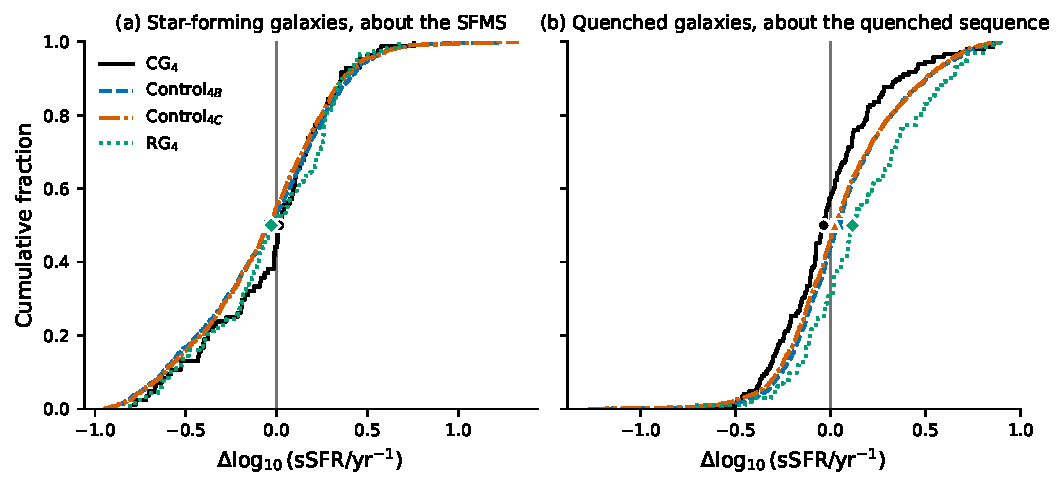
\includegraphics[width=0.9\textwidth]{main_sequence_residuals.pdf}
  \caption{Cumulative distributions of the sSFR residuals of (a) star-forming galaxies about the order-2 star-forming main sequence and (b) quenched galaxies about the order-4 quenched sequence, both fitted to the SDSS non-AGN reference sample. Zero marks the fitted relation; filled symbols mark the sample medians. MPA--JHU sSFRs of quenched galaxies are largely \(D_n4000\)-calibrated, so panel (b) is weakly informative.}
  \label{fig:supp_sfms_residuals}
\end{figure*}

\section{Optical-colour diagnostics}

The retained colour-analysis matches include 110 of 248 galaxies in CG$_4$, 931 of 2792 galaxies in Control$_{4B}$, 1153 of 2812 galaxies in Control$_{4C}$, 102 of 224 galaxies in RG$_4$. The colour analysis requires successful matched-photometry retention and the covariates used below; the fractions retained are 44.4\% in CG4, 33.3\% in Control4B, 41.0\% in Control4C, 45.5\% in RG4. The subset is not representative of the full catalogues: matched galaxies are systematically less massive, more actively star-forming, and more frequently satellites than unmatched galaxies (Fig.~\ref{fig:supp_colour_selection}).

The raw colour--mass fits do not show a single common relation for every sample: common slopes are rejected in all four colours, with the directional slope differences having small adjusted p-values mainly in the bluer colours and depending on the comparison catalogue. In the satellite-only comparison, the fitted offsets and slopes likewise depend on the control definition. In cluster-robust satellite fits, the negative \CG{} coefficients in the pooled mass- and redshift-adjusted comparison are weak, and adding morphology and sSFR class does not reveal a clear negative coefficient. These coefficients remain control-sample dependent, with non-uniform split-sample behaviour (Fig.~\ref{fig:supp_colour_coefficients}). They therefore do not identify a global colour shift or a simple interaction-triggered star-forming population.

\begin{figure*}
  \centering
  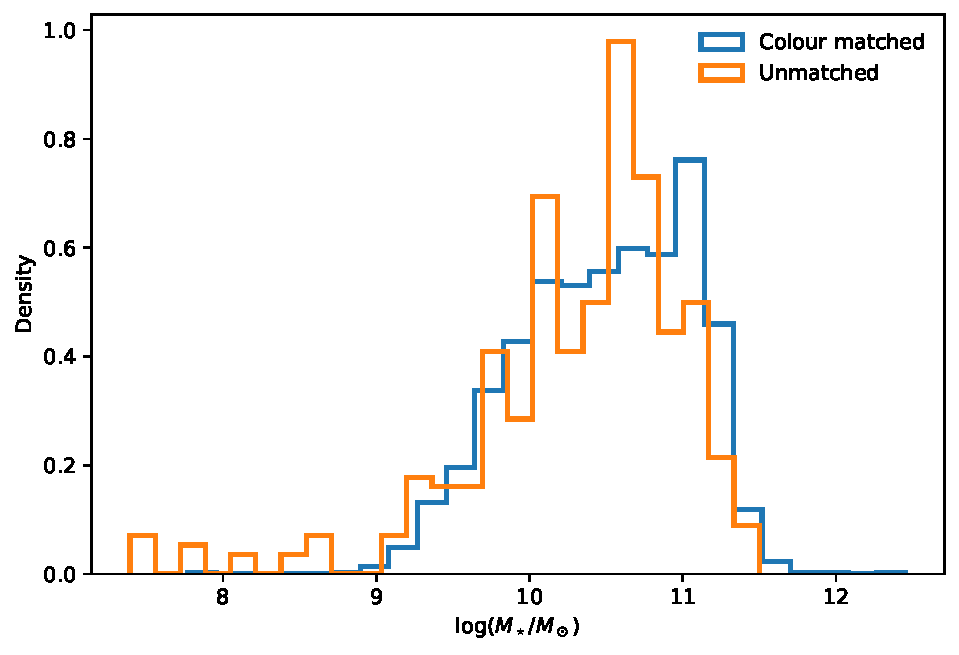
\includegraphics[width=0.9\textwidth]{fig_colour_matched_selection_bias.pdf}
  \caption{Selection diagnostics for the matched-photometry colour subset. The plotted comparisons show how galaxies retained for the colour analysis differ from those not retained in the audited quantities.}
  \label{fig:supp_colour_selection}
\end{figure*}

\begin{figure*}
  \centering
  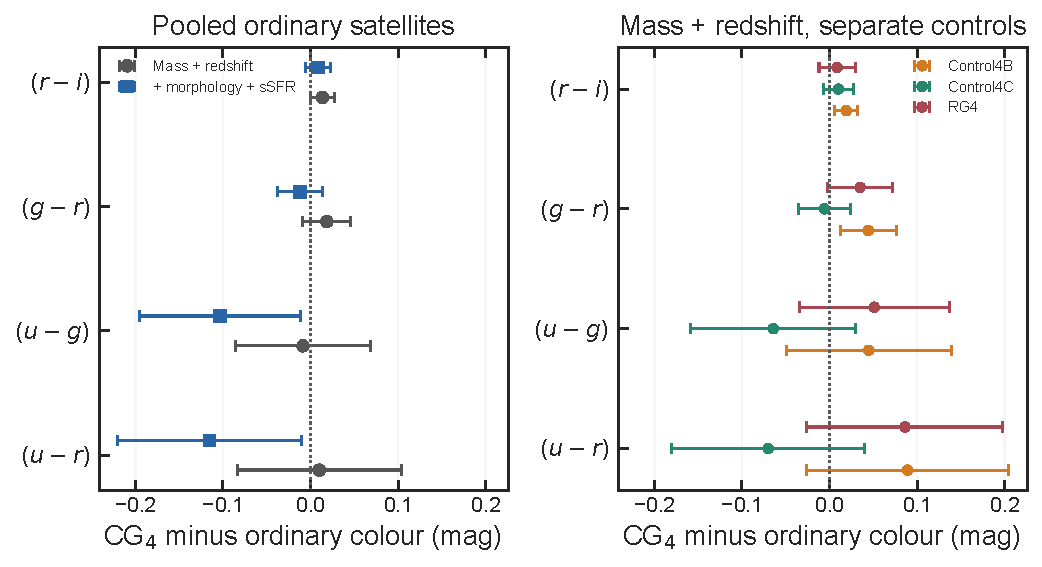
\includegraphics[width=\textwidth]{colour_robustness_coefficients.pdf}
  \caption{Robustness of the satellite colour coefficients. Left: pooled ordinary-group comparison before and after controlling for GZ1 E/S morphology and sSFR class. Right: mass- and redshift-adjusted comparisons against each control catalogue separately. Points show the \CG{} minus ordinary-group coefficient and bars show 95\% confidence intervals; negative values indicate bluer \CG{} satellites.}
  \label{fig:supp_colour_coefficients}
\end{figure*}

\begin{figure*}
  \centering
  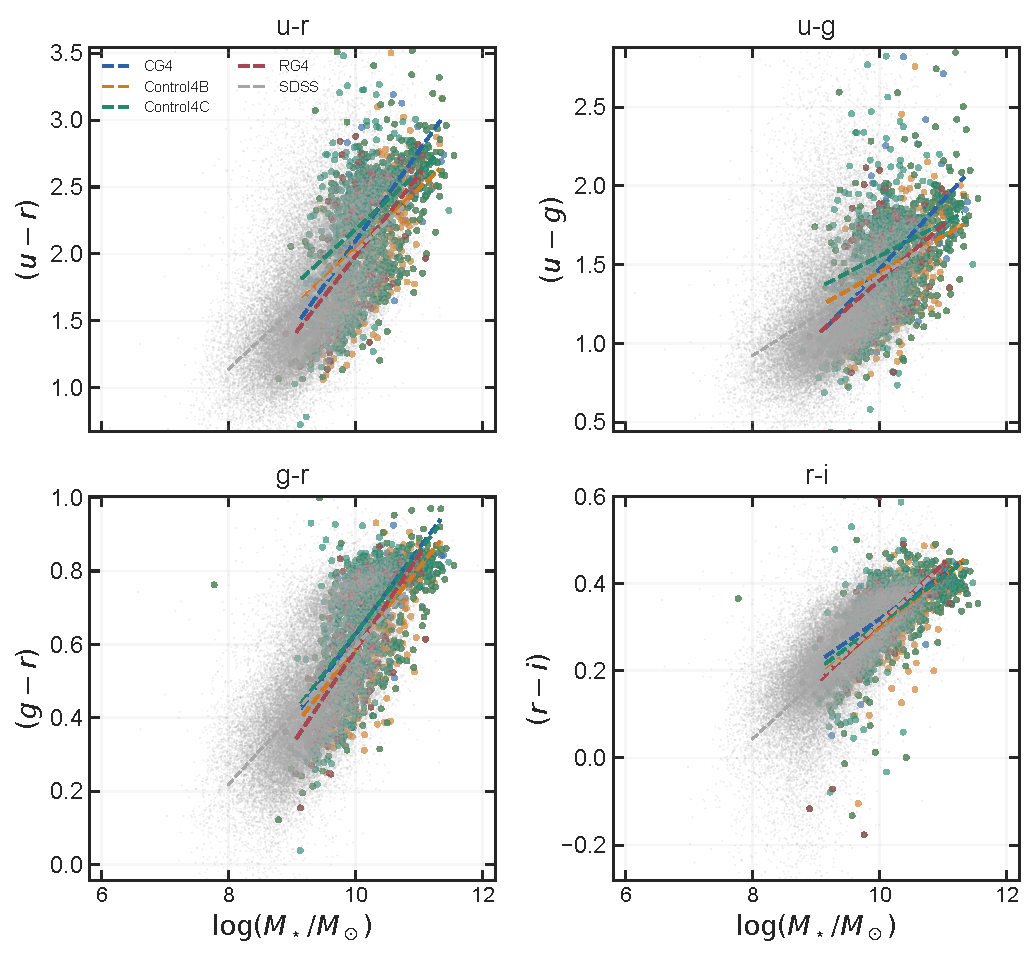
\includegraphics[width=\textwidth]{colour_mass_relations.pdf}
  \caption{Colour--stellar-mass relations in the four catalogues. These raw relations motivate the control-specific adjusted comparisons rather than a single pooled interpretation.}
  \label{fig:supp_colour_mass}
\end{figure*}

\begin{figure*}
  \centering
  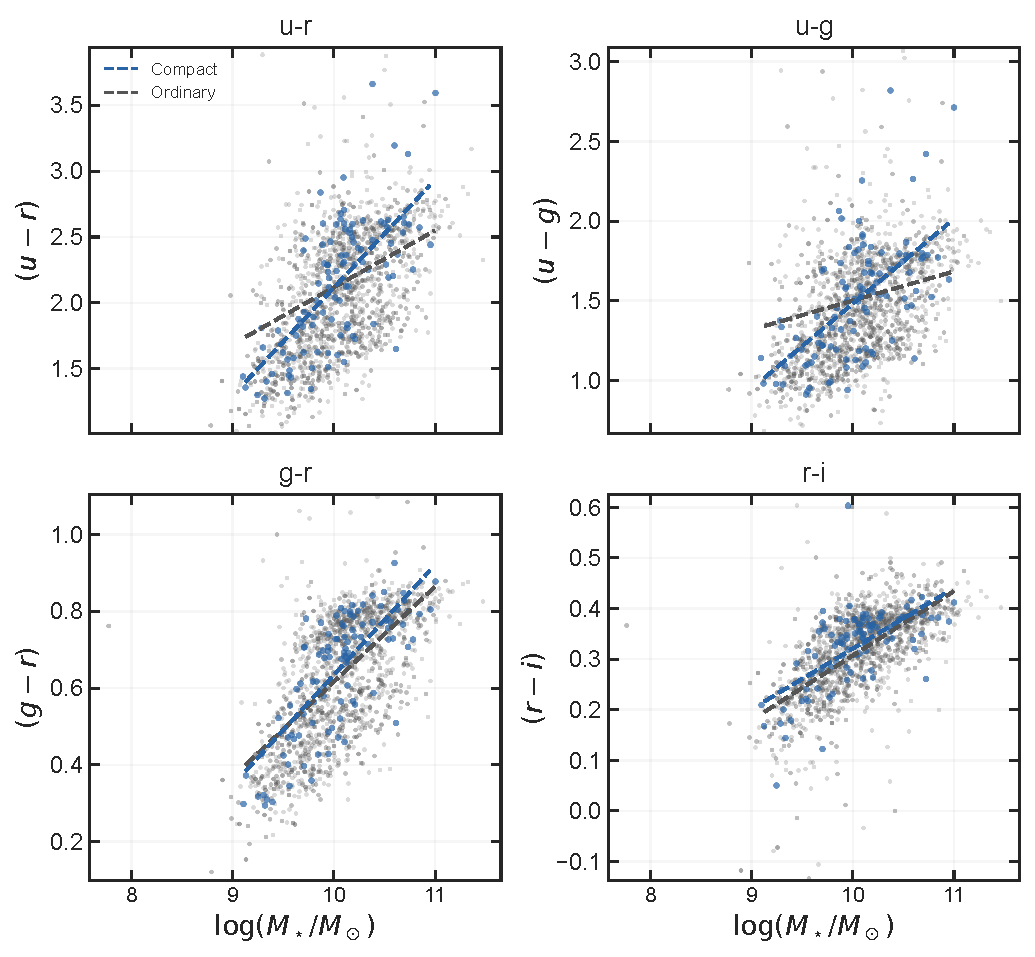
\includegraphics[width=\textwidth]{satellite_colour_mass_environment.pdf}
  \caption{Satellite colour--mass relations split by environment. The offsets and slopes depend on the comparison catalogue.}
  \label{fig:supp_satellite_colour}
\end{figure*}

\begin{figure*}
  \centering
  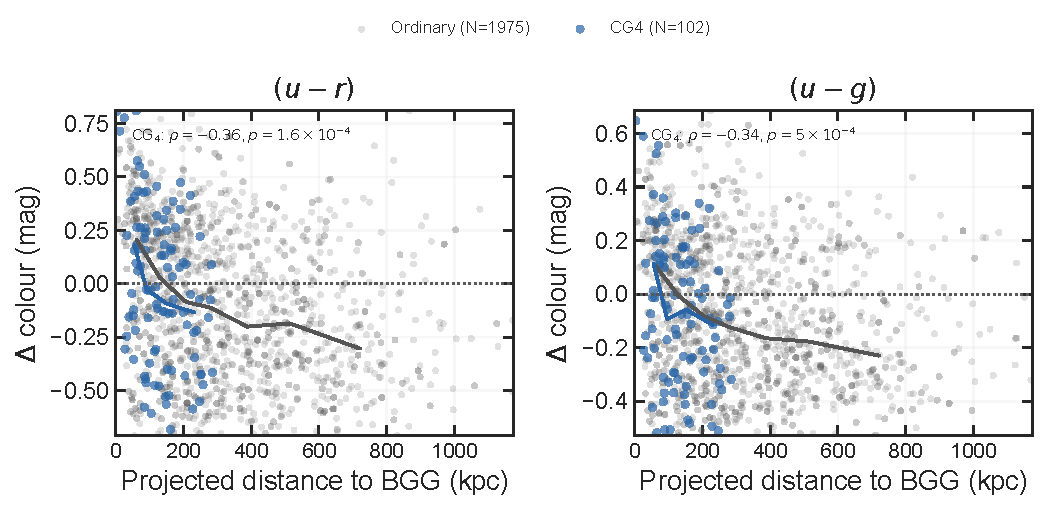
\includegraphics[width=\textwidth]{colour_residual_distance.pdf}
  \caption{Colour residuals versus projected BGG-centric distance. These trends are exploratory and inherit the matched-photometry selection described above.}
  \label{fig:supp_colour_radius}
\end{figure*}

\clearpage
\section{Pooled adjusted models}

For a compact summary across the heterogeneous control definitions, the article also fits binomial models to a pooled catalogue. Because the control catalogues overlap heavily, the control side is first deduplicated by SDSS object identifier and standard errors are clustered by physical Lim group. The common adjustment set contains stellar mass, redshift, satellite/BGG rank, group luminosity, and velocity dispersion. The figure below visualises the coefficients tabulated in Appendix H of the article. The pooled model is a summary, not a replacement for the separate-control contrasts: it reinforces the satellite E-class morphology shift, whereas the quenched estimate changes across controls and is not reproduced by the matched comparison.

\begin{center}
  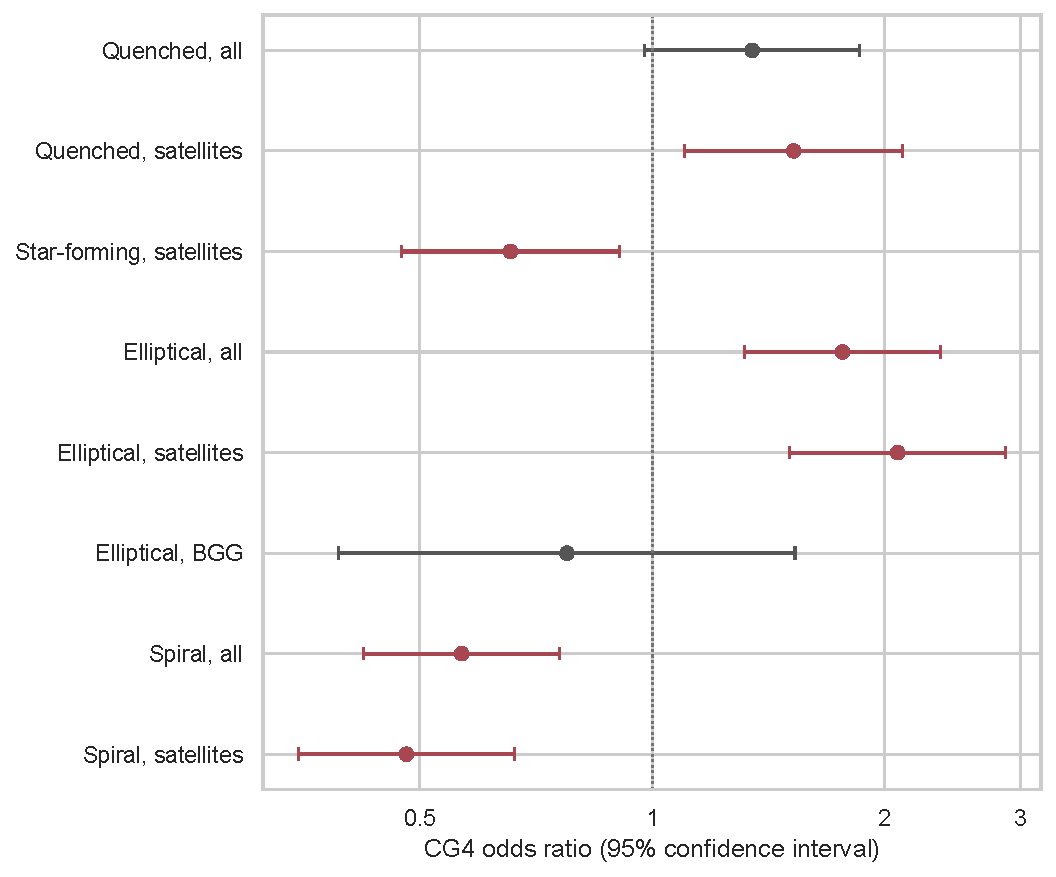
\includegraphics[width=\columnwidth]{fig_specialness_logistic_coefficients.pdf}
  \par\smallskip
  \begin{minipage}{\columnwidth}\small
  \textbf{Fig. S.7.} Adjusted \CG{} odds ratios from the pooled models. The GZ1 E-class outcomes refer to the smooth early-type-like GZ1 class, not to a physically pure sample of classical ellipticals. Points are odds ratios and bars are 95\% confidence intervals; the vertical line marks no difference.
  \end{minipage}
\end{center}

\clearpage
\section{Additional environmental diagnostics}

The distance-to-BGG, magnitude-gap, and luminosity-dominance screens are retained here because they are useful provenance checks but do not add a control-independent signal to the article. Satellite sSFR shows no consistent monotonic dependence on projected BGG distance across the four samples. Binary dominance splits and further subdivision by BGG morphology produce small, heterogeneous subsets; their occasional low p-values do not survive as a coherent compact-group effect. Likewise, magnitude-gap differences are sensitive to the control definition. These diagnostics support the article's choice to retain the continuous group-scale screen and projected phase-space result as the more interpretable summaries.

The optical-colour panels above give the corresponding full distributional diagnostics: matched-photometry retention is selective, and fitted offsets depend on the control definition and split sample.


\section{Size-model comparison by control}

\begin{figure}[H]
  \centering
  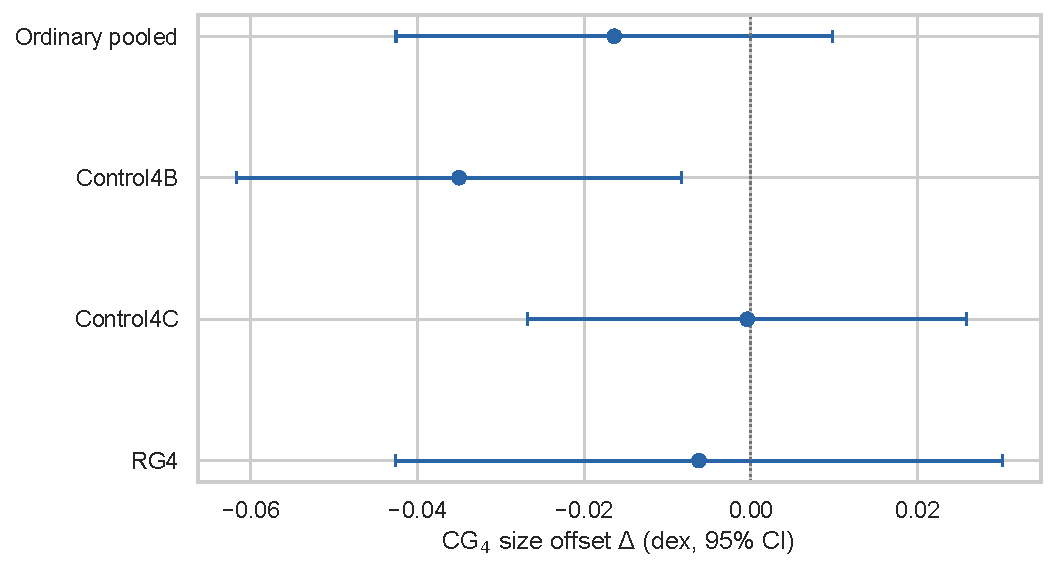
\includegraphics[width=\columnwidth]{size_forest_per_control.pdf}
  \caption{Group-adjusted \CG{} size coefficients against the deduplicated pooled controls and each control catalogue separately. Every model uses the article's main adjustment set: stellar mass, redshift, rank, group luminosity, and velocity dispersion, with physical-group-clustered uncertainties. Bars are 95\% confidence intervals; negative values denote smaller \CG{} effective radii at fixed covariates.}
  \label{fig:supp_size_per_control}
\end{figure}


\end{document}